\documentclass[12pt]{article}

%% packages
\usepackage{color,verbatim,Sweave,url,xargs,amsmath,graphicx}
\usepackage[left=0.5in, right=.5in, top=1in, bottom=.75in]{geometry}
% \usepackage{times}
\usepackage{multicol}
\usepackage{enumitem}
\usepackage{arev}
\usepackage{fancyhdr}


\setkeys{Gin}{width=0.5\linewidth}

%% new environments
\newenvironment{question}{\item}{\vfill}
\newenvironment{solution}{\comment}{\endcomment}
\newenvironment{answerlist}{\renewcommand{\labelenumi}{(\alph{enumi})}\begin{samepage}\begin{enumerate}[topsep=0pt,itemsep=-1ex,partopsep=1ex,parsep=1ex]}{\end{enumerate}\end{samepage}}
%%\newenvironment{answerlist}{\setlength{\itemsep}{0pt}\setlength{\parskip}{0pt}\renewcommand{\labelenumi}{(\alph{enumi})}\begin{multicols}{2}\begin{enumerate}}{\end{enumerate}\end{multicols}}
%% \newenvironment{answerlist}{\renewcommand{\labelenumi}{(\alph{enumi})}\begin{multicols}{2}\begin{enumerate}}{\end{enumerate}\end{multicols}}



%% paragraphs
\setlength{\parskip}{0.7ex plus0.1ex minus0.1ex}
\setlength{\parindent}{0em}

%% compatibility with pandoc
\providecommand{\tightlist}{\setlength{\itemsep}{0pt}\setlength{\parskip}{0pt}}

% %% fonts: Helvetica
% \renewcommand{\sfdefault}{phv}
% \IfFileExists{sfmath.sty}{
%   \RequirePackage{sfmath}
%   \renewcommand{\rmdefault}{phv}
% }{}



% %% headings
% \markboth{\textnormal{\bf \large Statistics Exam: \myID}}%
% {\textnormal{\bf \large Statistics Exam: \myID}}
% \pagestyle{myheadings}

\begin{document}

\pagestyle{fancy}
\fancyhf{}
\rhead{Precalculus Unit 4}
\lhead{\sc{Fusion Academy}}
\chead{QUESTIONS}
\rfoot{Page \thepage}
\setlength{\headheight}{15pt}


%% title page
% \thispagestyle{empty}
% {\sf
% \textbf{\LARGE{Fusion Academy}}

% \textbf{\large{Statistics Exam \myDate \hfill Exam ID \myID}}


\vspace*{0.1cm}

\begin{flushright}
\begin{tabular}{p{14cm}}
\textbf{\Large{Name:}} \hrule \\[1.5cm]
\textbf{\Large{Date:}} \hrule \\[0.5cm]
% \textbf{Signature:} \hrule  \\[1.5cm]
\end{tabular}
\end{flushright}
% 
% \vspace*{1cm}

% \newpage

\begin{enumerate}

\begin{question}
Solve the following system.

\[\begin{aligned}
- 4 x - 7 y&=29\\
- x + 2 y&=-4
\end{aligned}\]
\end{question}

\begin{solution}
\[\begin{aligned}
x&=-2\\
y&=-3
\end{aligned}\]
\end{solution}



\begin{question}
Solve the following system.

\[\begin{aligned}
20 x + 10 y&=148\\
4 x + 2 y&=-16
\end{aligned}\]
\end{question}

\begin{solution}
The system is inconsistent. The two equations represent two parallel
lines, so no pair of \(x\) and \(y\) can satisfy both equations.
\end{solution}



\begin{question}
Solve the following system.

\[\begin{aligned}
- 7 x - 5 y&=-55\\
14 x + 10 y&=110
\end{aligned}\]
\end{question}

\begin{solution}
The system is undetermined. Both equations describe the same line, so
there are infinite pairs of \(x\) and \(y\) that satisfy the system.
Notice that ``infinite'' does not mean ``all'', \emph{most} pairs of
\(x\) and \(y\) are not solutions.
\end{solution}



\begin{question}
Solve the following system.

\[\begin{aligned}
- 8 x - 3 y - 5 z&=30\\
8 x - 6 y + 6 z&=-76\\
2 x - 2 y + 6 z&=-66
\end{aligned}\]
\end{question}

\begin{solution}
\[\begin{aligned}
x&=1\\
y&=4\\
z&=-10
\end{aligned}\]
\end{solution}



\begin{question}
Solve the following system.

\[\begin{aligned}
- 16 x + 14 y - 14 z&=72\\
- 3 x + y + 12 z&=-6\\
19 x - 15 y + 2 z&=-66
\end{aligned}\]
\end{question}

\begin{solution}
The system is undetermined. There are infinite solutions. This might be
because two planes are equivalent, or because all three planes meet in a
line, or because all three planes are equivalent.
\end{solution}



\begin{question}
Solve the system of equations.

\[\begin{aligned}
- 2 x^{2} + 4 x + y &= 168 \\
2 x - y &= 8
\end{aligned}\]
\end{question}

\begin{solution}
There are two solutions.

\[(8,8) \text{ and } (11,14) \]

This system represents a parabola and a line.

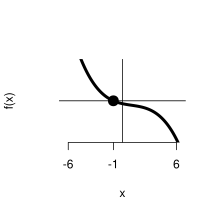
\includegraphics{unnamed-chunk-2-1.pdf}\\
\end{solution}



\begin{question}
Solve the system of equations.

\[\begin{aligned}
- 3 x^{2} + 6 x + y &= 28 \\
12 x - y &= -25
\end{aligned}\]
\end{question}

\begin{solution}
There is one solution.

\[(-1,13)\]

This system represents a parabola and a tangent line.

\includegraphics{unnamed-chunk-2-1-2.pdf}\\
\end{solution}



\begin{question}
Solve the system of equations.

\[\begin{aligned}
- 10 x^{2} + 20 x + y &= 31 \\
80 x - y &= 31
\end{aligned}\]
\end{question}

\begin{solution}
There is no solution.

This system represents a parabola and a non-intersecting line.

\includegraphics{unnamed-chunk-2-1-3.pdf}\\
\end{solution}



\begin{question}
A thief is filling her backpack with two types of valuable substances.
She can carry up to 30 kg, and her backpack can fit up to 10 liters.

Each bag of \(X\) has a weight of 3 kg, volume of 0.4 L, and value of 10
thousand USD.

Each bag of \(Y\) has a weight of 0.8 kg, volume of 0.6 L, and value of
5 thousand USD.

There is no requirement to take full bags, so the thief can opt for a
fraction of a bag.

How many bags of each should the thief take to maximize her profit?
\end{question}

\begin{solution}
The thief should take 6.76 bags of \(X\) and 12.16 bags of \(Y\). We can
use linear programming to see this.

We write a weight inequality. \[3x+0.8y \le 30\] We write a volume
inequality. \[0.4x+0.6y \le 10\] We graph the two inequalities, shading
the feasible region.

\includegraphics{unnamed-chunk-1-1.pdf}\\

There are three vertices of interest. \[(0,16.67) \] \[(6.76,12.16) \]
\[(10,0)\]

We write a profit function (the objective function).
\[P(x,y) = 10x+5y \]

We determine the profits. \[P(0,16.67)=83.33 \]
\[P(6.76,12.16)=128.38 \] \[P(10,0)=100 \] Thus, the thief should take
6.76 bags of \(X\) and 12.16 bags of \(Y\).
\end{solution}



\begin{question}
Determine the product of the matrix multiplication.

\[\left[\begin{matrix}-1 & 4\\-8 & 0\end{matrix}\right] \cdot \left[\begin{matrix}-2 & 5 & 2\\2 & -3 & 6\end{matrix}\right]\]
\end{question}

\begin{solution}
The answer:
\[\left[\begin{matrix}10 & -17 & 22\\16 & -40 & -16\end{matrix}\right]\]

The work:

1st row and 1st column\ldots{} \((-1)(-2)+(4)(2) = 10\)

1st row and 2nd column\ldots{} \((-1)(5)+(4)(-3) = -17\)

1st row and 3rd column\ldots{} \((-1)(2)+(4)(6) = 22\)

2nd row and 1st column\ldots{} \((-8)(-2)+(0)(2) = 16\)

2nd row and 2nd column\ldots{} \((-8)(5)+(0)(-3) = -40\)

2nd row and 3rd column\ldots{} \((-8)(2)+(0)(6) = -16\)
\end{solution}



\begin{question}
Find the multiplicative inverse of matrix \(A\).
\[A = \left[\begin{matrix}4 & 1 & 0\\5 & 3 & 3\\5 & 4 & 4\end{matrix}\right]\]
\end{question}

\begin{solution}
The answer:
\[\left[\begin{matrix}0 & \frac{4}{5} & - \frac{3}{5}\\1 & - \frac{16}{5} & \frac{12}{5}\\-1 & \frac{11}{5} & - \frac{7}{5}\end{matrix}\right]\]
\end{solution}


\end{enumerate}

\newpage

\renewenvironment{question}{\comment}{\endcomment}
\renewenvironment{solution}{\item}{\vfill}


\chead{SOLUTIONS}

\begin{enumerate}

\begin{question}
Solve the following system.

\[\begin{aligned}
- 4 x - 7 y&=29\\
- x + 2 y&=-4
\end{aligned}\]
\end{question}

\begin{solution}
\[\begin{aligned}
x&=-2\\
y&=-3
\end{aligned}\]
\end{solution}



\begin{question}
Solve the following system.

\[\begin{aligned}
20 x + 10 y&=148\\
4 x + 2 y&=-16
\end{aligned}\]
\end{question}

\begin{solution}
The system is inconsistent. The two equations represent two parallel
lines, so no pair of \(x\) and \(y\) can satisfy both equations.
\end{solution}



\begin{question}
Solve the following system.

\[\begin{aligned}
- 7 x - 5 y&=-55\\
14 x + 10 y&=110
\end{aligned}\]
\end{question}

\begin{solution}
The system is undetermined. Both equations describe the same line, so
there are infinite pairs of \(x\) and \(y\) that satisfy the system.
Notice that ``infinite'' does not mean ``all'', \emph{most} pairs of
\(x\) and \(y\) are not solutions.
\end{solution}



\begin{question}
Solve the following system.

\[\begin{aligned}
- 8 x - 3 y - 5 z&=30\\
8 x - 6 y + 6 z&=-76\\
2 x - 2 y + 6 z&=-66
\end{aligned}\]
\end{question}

\begin{solution}
\[\begin{aligned}
x&=1\\
y&=4\\
z&=-10
\end{aligned}\]
\end{solution}



\begin{question}
Solve the following system.

\[\begin{aligned}
- 16 x + 14 y - 14 z&=72\\
- 3 x + y + 12 z&=-6\\
19 x - 15 y + 2 z&=-66
\end{aligned}\]
\end{question}

\begin{solution}
The system is undetermined. There are infinite solutions. This might be
because two planes are equivalent, or because all three planes meet in a
line, or because all three planes are equivalent.
\end{solution}



\begin{question}
Solve the system of equations.

\[\begin{aligned}
- 2 x^{2} + 4 x + y &= 168 \\
2 x - y &= 8
\end{aligned}\]
\end{question}

\begin{solution}
There are two solutions.

\[(8,8) \text{ and } (11,14) \]

This system represents a parabola and a line.

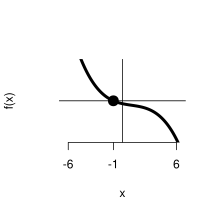
\includegraphics{unnamed-chunk-2-1.pdf}\\
\end{solution}



\begin{question}
Solve the system of equations.

\[\begin{aligned}
- 3 x^{2} + 6 x + y &= 28 \\
12 x - y &= -25
\end{aligned}\]
\end{question}

\begin{solution}
There is one solution.

\[(-1,13)\]

This system represents a parabola and a tangent line.

\includegraphics{unnamed-chunk-2-1-2.pdf}\\
\end{solution}



\begin{question}
Solve the system of equations.

\[\begin{aligned}
- 10 x^{2} + 20 x + y &= 31 \\
80 x - y &= 31
\end{aligned}\]
\end{question}

\begin{solution}
There is no solution.

This system represents a parabola and a non-intersecting line.

\includegraphics{unnamed-chunk-2-1-3.pdf}\\
\end{solution}



\begin{question}
A thief is filling her backpack with two types of valuable substances.
She can carry up to 30 kg, and her backpack can fit up to 10 liters.

Each bag of \(X\) has a weight of 3 kg, volume of 0.4 L, and value of 10
thousand USD.

Each bag of \(Y\) has a weight of 0.8 kg, volume of 0.6 L, and value of
5 thousand USD.

There is no requirement to take full bags, so the thief can opt for a
fraction of a bag.

How many bags of each should the thief take to maximize her profit?
\end{question}

\begin{solution}
The thief should take 6.76 bags of \(X\) and 12.16 bags of \(Y\). We can
use linear programming to see this.

We write a weight inequality. \[3x+0.8y \le 30\] We write a volume
inequality. \[0.4x+0.6y \le 10\] We graph the two inequalities, shading
the feasible region.

\includegraphics{unnamed-chunk-1-1.pdf}\\

There are three vertices of interest. \[(0,16.67) \] \[(6.76,12.16) \]
\[(10,0)\]

We write a profit function (the objective function).
\[P(x,y) = 10x+5y \]

We determine the profits. \[P(0,16.67)=83.33 \]
\[P(6.76,12.16)=128.38 \] \[P(10,0)=100 \] Thus, the thief should take
6.76 bags of \(X\) and 12.16 bags of \(Y\).
\end{solution}



\begin{question}
Determine the product of the matrix multiplication.

\[\left[\begin{matrix}-1 & 4\\-8 & 0\end{matrix}\right] \cdot \left[\begin{matrix}-2 & 5 & 2\\2 & -3 & 6\end{matrix}\right]\]
\end{question}

\begin{solution}
The answer:
\[\left[\begin{matrix}10 & -17 & 22\\16 & -40 & -16\end{matrix}\right]\]

The work:

1st row and 1st column\ldots{} \((-1)(-2)+(4)(2) = 10\)

1st row and 2nd column\ldots{} \((-1)(5)+(4)(-3) = -17\)

1st row and 3rd column\ldots{} \((-1)(2)+(4)(6) = 22\)

2nd row and 1st column\ldots{} \((-8)(-2)+(0)(2) = 16\)

2nd row and 2nd column\ldots{} \((-8)(5)+(0)(-3) = -40\)

2nd row and 3rd column\ldots{} \((-8)(2)+(0)(6) = -16\)
\end{solution}



\begin{question}
Find the multiplicative inverse of matrix \(A\).
\[A = \left[\begin{matrix}4 & 1 & 0\\5 & 3 & 3\\5 & 4 & 4\end{matrix}\right]\]
\end{question}

\begin{solution}
The answer:
\[\left[\begin{matrix}0 & \frac{4}{5} & - \frac{3}{5}\\1 & - \frac{16}{5} & \frac{12}{5}\\-1 & \frac{11}{5} & - \frac{7}{5}\end{matrix}\right]\]
\end{solution}


\end{enumerate}

\end{document}
